\documentclass{beamer}

\usepackage{amsmath}
\usepackage{textcomp}
\usepackage{listings}
\usepackage{lmodern}
\usepackage{hyperref}
\usepackage[T1]{fontenc}
\usepackage{tikz}
\usepackage{anyfontsize}

% Required for biblatex, but also adds functionality for quotation
\usepackage{csquotes}

% Jason's bibliography format
% % Credit to Gabriel Devenyi for this bibliography cfg:
% % github.com/gdevenyi/mcmaster.latex
% \usepackage[
%   style=numeric-comp,
%   backend=biber,
%   sorting=none,
%   backref=true,
%   maxnames=99,
%   alldates=iso,
%   seconds=true
% ]{biblatex} % bibliography
% \addbibresource{references.bib}
\usepackage[round]{natbib}
\bibliographystyle{plainnat}
\setcitestyle{yysep={;}}
\defcitealias{ISTQB}{Hamburg and Mogyorodi}
\newcommand{\citetISTQB}{\citetalias{ISTQB} (\citeyear{ISTQB})}
\newcommand{\citepISTQB}{\citepalias[\citeyear{ISTQB}]{ISTQB}}
\newcommand{\citealpISTQB}{\citetalias{ISTQB}, \citeyear{ISTQB}}

% For directory trees
\usepackage{dirtree}

\lstset{
    language=[latex]tex,
    breaklines=true}

\usetheme{Madrid}

\setbeamertemplate{caption}{\centering\insertcaption\par}

\def\checkmark{\tikz\fill[scale=0.4](0,.35) -- (.25,0) -- (1,.7) -- (.25,.15) -- cycle;} 

\newif\ifnotpaper

\def\litStd{If the field of software engineering holds code to a high standard
    in terms of clarity, consistency, and robustness, then the literature that
    supports code development should be held to this same standard!}

\def\badTaxonomies{Unfortunately, a search for a systematic, rigorous, and
    complete taxonomy for software testing revealed that the existing ones are
    inadequate and incomplete:

    \begin{itemize}
        \item \ifnotpaper\else Tebes et al. \fi\citet{TebesEtAl2020a} focus on
              \emph{parts} of the testing process (e.g., test goal, testable entity),
        \item \ifnotpaper\else Souza et al. \fi\citet{SouzaEtAl2017} prioritize
              organizing testing approaches over defining them, and
        \item \ifnotpaper\else Unterkalmsteiner et al. \fi\citet{UnterkalmsteinerEtAl2014}
              focus on the ``information linkage or transfer'' \citetext{p.~A:6}
              between requirements engineering and software testing.
    \end{itemize}}
\notpapertrue

\title[Testing Terminology]{Putting Software Testing Terminology to the Test}
\subtitle{M.A.Sc. Seminar}
\author[Samuel Crawford]{Samuel Crawford, B.Eng.}

% Committee
% \begin{itemize}
%     \item \emph{Supervisor}: Dr.~Jacques Carette
%     \item \emph{Supervisor}: Dr.~Spencer Smith
%     \item Dr.~Ned Nedialkov
%     \item Dr.~Richard Paige
% \end{itemize}

\institute[McMaster University]{McMaster University\\Department of Computing and Software}
\date{Fall 2024}

\AtBeginSection[]
{
  \begin{frame}
    \frametitle{Table of Contents}
    \tableofcontents[currentsection]
  \end{frame}
}

\begin{document}

% From https://tex.stackexchange.com/a/42826/192195
\NewDocumentCommand{\ShowListingForLineNumber}{s O{1.0} m m}{
    \IfBooleanTF{#1}{\vspace{-#2\baselineskip}}{}
    \lstinputlisting[
        style=MyListStyle,
        linerange={#3-#3},
        firstnumber=#3,
    ]{#4}
}

%%%%%%%%%%%%%%%%%%%%%%%%%%%%%%%%%%%%%%%%%%%%%%%%%%%%%%%%%%%%%%%%%%%%%%%%%%%%%%%
%% TITLE PAGE
%%%%%%%%%%%%%%%%%%%%%%%%%%%%%%%%%%%%%%%%%%%%%%%%%%%%%%%%%%%%%%%%%%%%%%%%%%%%%%%
\frame{\titlepage}

%%%%%%%%%%%%%%%%%%%%%%%%%%%%%%%%%%%%%%%%%%%%%%%%%%%%%%%%%%%%%%%%%%%%%%%%%%%%%%%
%% TABLE OF CONTENTS
%%%%%%%%%%%%%%%%%%%%%%%%%%%%%%%%%%%%%%%%%%%%%%%%%%%%%%%%%%%%%%%%%%%%%%%%%%%%%%%

\begin{frame}
    \frametitle{Table of Contents}
    \tableofcontents
\end{frame}

%%%%%%%%%%%%%%%%%%%%%%%%%%%%%%%%%%%%%%%%%%%%%%%%%%%%%%%%%%%%%%%%%%%%%%%%%%%%%%%
%% INTRODUCTION
%%%%%%%%%%%%%%%%%%%%%%%%%%%%%%%%%%%%%%%%%%%%%%%%%%%%%%%%%%%%%%%%%%%%%%%%%%%%%%%
\section{Introduction}

\subsection{The Need for Standardized Terminology}

\begin{frame}
    \frametitle{The Need for Standardized Terminology}
    \begin{itemize}
        \item Since engineering is applied science, and scientific fields use
              precise terminology, the same should be true of software engineering
        \item <2-> Imagine if other fields used unclear, inconsistent, and
              incorrect terminology:
              \begin{itemize}
                  \item Force
                  \item Isotope
                  \item Phalange
              \end{itemize}
    \end{itemize}
    \begin{exampleblock}<3->{}
        {\large \litStd{}}
        % \vspace{3mm}
        % \hspace\fill{\small--- Dr.~Jacques Carette}
    \end{exampleblock}
\end{frame}

\begin{frame}
    \frametitle{Improved Communication}
    \begin{columns}[T]
        \begin{column}{.5\textwidth}
            \begin{center}
                \huge Interorganizational

                \normalsize Schools, companies, etc.

                \vspace{5mm}

                % Based on code frustratingly generated by ChatGPT
                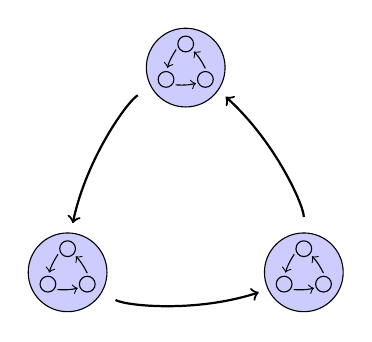
\begin{tikzpicture}

                    % Define coordinates of the triangle's vertices
                    \coordinate (A) at (0, 0);
                    \coordinate (B) at (3, 0);
                    \coordinate (C) at (1.5, 2.6);
                    \coordinate (D) at (1.5, 0.86667);

                    % Draw circles at each vertex without labels
                    \draw[fill=blue!20] (A) circle [radius=0.5];
                    \draw[fill=blue!20] (B) circle [radius=0.5];
                    \draw[fill=blue!20] (C) circle [radius=0.5];

                    % Draw arrows as arcs
                    \draw[->, thick, shorten <= 20pt] (B) arc (0:48:3cm);
                    \draw[->, thick, shorten <= 20pt] (C) arc (120:168:3cm);
                    \draw[->, thick, shorten <= 20pt] (A) arc (240:288:3cm);

                    % Small diagrams inside each circle
                    \only<2->{
                        \foreach \x in {A,B,C} {
                                \begin{scope}[shift={(\x)}, scale=0.2] % Scaling down and shifting to position A
                                    \coordinate (D) at (-1.25, -0.75);
                                    \coordinate (E) at (1.25, -0.75);
                                    \coordinate (F) at (0, 1.5);
                                    \draw[fill=blue!20] (D) circle [radius=0.5];
                                    \draw[fill=blue!20] (E) circle [radius=0.5];
                                    \draw[fill=blue!20] (F) circle [radius=0.5];
                                    \draw[->, shorten <= 4pt] (E) arc (0:45:2.5cm);
                                    \draw[->, shorten <= 4pt] (F) arc (120:165:2.5cm);
                                    \draw[->, shorten <= 4pt] (D) arc (240:285:2.5cm);
                                \end{scope}
                            }
                    }
                \end{tikzpicture}
            \end{center}
        \end{column}
        \begin{column}<2->{.5\textwidth}
            \begin{center}
                \huge Intraorganizational \normalsize
            \end{center}

            ``Complete testing'' could require the tester to:
            \begin{itemize}
                \item discover ``every bug in the product'',
                \item exhaust the time allocated to the testing phase,
                \item implement every test previously agreed upon,
                \item \dots{} \citep[p.~7]{KanerEtAl2011}
            \end{itemize}
        \end{column}
    \end{columns}
\end{frame}

\subsection{The Lack of Standardized Terminology}

\begin{frame}
    \frametitle{The Lack of Standardized Terminology}
    \framesubtitle{``The Problem''}
    \begin{itemize}
        \item \badTaxonomies{}
    \end{itemize}
\end{frame}

%%%%%%%%%%%%%%%%%%%%%%%%%%%%%%%%%%%%%%%%%%%%%%%%%%%%%%%%%%%%%%%%%%%%%%%%%%%%%%%
%% PROJECT
%%%%%%%%%%%%%%%%%%%%%%%%%%%%%%%%%%%%%%%%%%%%%%%%%%%%%%%%%%%%%%%%%%%%%%%%%%%%%%%

\section{Project}

\begin{frame}
    \frametitle{The Problem with Testing Literature}
    \framesubtitle{Unstandardized Standards}
\end{frame}

\subsection{Drasil}

% \begin{frame}
%     \frametitle{Drasil}
%     \framesubtitle{"Generate All The Things!"}
%     % TODO: "Generate All The Things!" is a beautifully appropriate tagline for Drasil
%     %       for a few reasons:
%     %                  1. What are "Things"? One may only think of "Things" as far as their knowledge and understanding allows them! You wouldn't be able to think of things without some sort of basis/constructive understanding/methodology to _get_ there, you can't _think of random phenomena_ (that's why they're phenomena).

%     \begin{itemize}
%         \item<2-> An exploration in software-related artifact generation for "well understood" domains \citep{KnowledgeCapture2021} through strong knowledge capture.
%             \begin{itemize}
%                 \item<3-> By unifying knowledge into a single framework with reusable composable units of knowledge, we eliminate code duplication, formally impose traceability and maintainability of knowledge (and software), and allow for easy knowledge transference.
%                 \item<4-> Knowledge organization and capture is of utmost importance, as it is the pathway for interpreters and Domain-Specific Languages (DSLs) to make appropriate usage of the knowledge captured.
%                 \item<5-> By creating different kinds of "printers", we can use a stable knowledge-base to generate software that solves "well understood" problems.
%             \end{itemize}
%         \item<6-> Drasil currently focuses on building research software, generating Software Requirement Specification documents (SRS) in both LaTeX and HTML (with MathJaX), code to solve a problem, README files, Makefiles, graphs, etc.
%     \end{itemize}
% \end{frame}

\begin{frame}
    \frametitle{Problem Statement}
    \begin{itemize}
        \item Currently, there is no way to verify Drasil's output
        \item <2-> Drasil is "tested" by comparing generated
              artifacts to \texttt{stable}
              \begin{columns}[T,onlytextwidth]
                  \begin{column}{.4\textwidth}
                      %   \begin{figure}
                      %       %   \vspace{-1mm}
                      %       \includegraphics[width=.8\textwidth]{assets/stable.png}
                      %       %   \vspace{-3mm}
                      %       \caption{Contents of \texttt{stable}}
                      %       \vspace{-1mm}
                      %   \end{figure}
                  \end{column}
                  \begin{column}{.6\textwidth}
                      %   \lstinputlisting[
                      %       title=An example log,
                      %       captionpos=b,
                      %       language={},
                      %       basicstyle=\tiny, % TODO: reduce font size?
                      %       breakatwhitespace=true,
                      %       showstringspaces=false
                      %   ]{assets/log.txt}
                      \vspace{-2mm}
                  \end{column}
              \end{columns}
        \item <3-> This does not actually say anything about Drasil's output!
    \end{itemize}
\end{frame}

\begin{frame}
    \frametitle{Purpose Statement}
    \begin{itemize}
        \item The purpose of this research is to implement test case generation
              to verify generated code
        \item These test cases will be generated from information within Drasil
        \item<2-> Why use test cases for verification as opposed to, say,
              consistency/correctness checks?
              \begin{enumerate}
                  \item<3-> A more well-defined, Master's level scope
                  \item<4-> Targets a more complex artifact that is harder to verify
                  \item<5-> Gives Drasil another "bragging point"!
              \end{enumerate}
    \end{itemize}
\end{frame}

\subsection{Why Test Generated Code?}

\begin{frame}
    \frametitle{Why Test Generated Code?}
    If the code is being generated from a stable knowledge base,
    then it should be correct. Why waste effort testing it?
    \begin{enumerate}
        \item<2-> The knowledge base is not actually "stable" yet
        \item<3-> There are plenty of places for a mistake to be introduced
              %, both by Drasil's developers and "end users"
        \item<4-> Testing provides a greater degree of confidence in
              Drasil's capabilities
        \item<5-> Generating code for testing allows for it to be done
              "properly" instead of taking shortcuts commonly taken by humans
    \end{enumerate}
\end{frame}

\subsection{Next Steps}

\begin{frame}
    \frametitle{Next Steps}
    2. Understand the manual artifact (and its components) well
    \begin{itemize}
        \item<2-> Understanding the problem domain lets one develop
              a solution that:
              \begin{itemize}
                  \item Makes use of all areas of the domain
                  \item Follows domain standards, including quality and terminology
              \end{itemize}
        \item<3-> There are specific areas of testing that need to be understood:
              \begin{itemize}
                  \item<4-> \textbf{Research Question \#1:}
                        What information is necessary for different types of testing?
                  \item<5-> \textbf{Research Question \#2:}
                        How can test cases be generated from information that currently
                        exists within Drasil?
                  \item<6-> \textbf{Research Question \#3:}
                        How can new information be added to facilitate the generation of
                        more types of testing?
              \end{itemize}
    \end{itemize}
    \onslide<7-|handout:1>\begin{exampleblock}{}
        {\large "The information you have should be just as useful for generating
            tests as it should be for manually running them."}
        \vspace{3mm}
        \hspace\fill{\small--- Dr.~Jacques Carette}
    \end{exampleblock}
\end{frame}

\begin{frame}
    \frametitle{Next Steps}
    3. Generate it!
    \begin{itemize}
        \item<2-> Test cases will then be written for:
              \begin{itemize}
                  \item Other variabilities of Projectile's Python implementation
                  \item Projectile's implementation in other languages
                  \item Other examples where code is generated: GlassBR, NoPCM,
                        DblPendulum, PD Controller \citep{HuntEtAl2021}
              \end{itemize}
        \item<3-> These test cases will also be added to Drasil's CI/CD
              to ensure that future changes preserve the code's functionality
    \end{itemize}
\end{frame}

%%%%%%%%%%%%%%%%%%%%%%%%%%%%%%%%%%%%%%%%%%%%%%%%%%%%%%%%%%%%%%%%%%%%%%%%%%%%%%%
%% ACKNOWLEDGEMENTS
%%%%%%%%%%%%%%%%%%%%%%%%%%%%%%%%%%%%%%%%%%%%%%%%%%%%%%%%%%%%%%%%%%%%%%%%%%%%%%%

\begin{frame}
    \frametitle{Acknowledgment}

    \begin{itemize}
        \item Dr.~Smith and Dr.~Carette have been great supervisors in the
              past and have, both then and now, provided me with valuable guidance
              and feedback
              \begin{itemize}
                  \item They have helped me refine the scope of this project
                  \item The project itself was originally posed by Dr.~Smith back
                        in 2020!
              \end{itemize}
        \item<2-> The format of this presentation was \emph{heavily} based on
              a previous presentation by Jason Balaci, who also provided a
              great thesis template
              % \item<2-> Dr.~Smith created the knowledge flow figure shown earlier
        \item<3-> The past and current Drasil team have created a truly amazing
              framework!
    \end{itemize}
\end{frame}

%%%%%%%%%%%%%%%%%%%%%%%%%%%%%%%%%%%%%%%%%%%%%%%%%%%%%%%%%%%%%%%%%%%%%%%%%%%%%%%
%% A FINAL THANK YOU
%%%%%%%%%%%%%%%%%%%%%%%%%%%%%%%%%%%%%%%%%%%%%%%%%%%%%%%%%%%%%%%%%%%%%%%%%%%%%%%

\begin{frame}
    \center
    \huge{Thank you!}\\
    \normalsize{Questions?}
\end{frame}

%%%%%%%%%%%%%%%%%%%%%%%%%%%%%%%%%%%%%%%%%%%%%%%%%%%%%%%%%%%%%%%%%%%%%%%%%%%%%%%
%% REFERENCES
%%%%%%%%%%%%%%%%%%%%%%%%%%%%%%%%%%%%%%%%%%%%%%%%%%%%%%%%%%%%%%%%%%%%%%%%%%%%%%%

\section{References}

\begin{frame}%[allowframebreaks]
    \frametitle{References}

    \bibliography{references}
\end{frame}

\end{document}
